% +--------------------------------------------------------------------+
% | Sample Chapter 3
% +--------------------------------------------------------------------+

\cleardoublepage

% +--------------------------------------------------------------------+
% | Replace "This is Chapter 3" below with the title of your chapter.
% | LaTeX will automatically number the chapters.
% +--------------------------------------------------------------------+
    %\renewcommand{\chaptername}{Part}
    %\renewcommand{\thechapter}{}
\chapter{Implementation}
\label{makereference}

\section{General overview of the system}
La cámara proporciona los pixeles de la imagen por bandas. Las primeras operaciones a realizar con estos datos son calcular la media, con ella la deviación y con esta la covarianza. Dadas la relativa simpleza de estas operaciones pero sus altos requisitos en memoria, estas tres operaciones son realizadas en una CPU y sus resultados enviados a la FPGA. La FPGA comenzará el cálculo de las operaciones posteriores solo cuando tenga los resultados completos de la covarianza.
Los datos calculados por la CPU son introducidos en la FPGA a traves de FIFOs.
La FPGA calculará entonces la inversa de la matriz. Mientras tanto la CPU tendrá que escribir las medias calculadas y los valores que había recibido anteriormente de la cámara, uno por uno. Cuando termine la inversa, la FPGA realizará las dos últimas multiplicaciones de matrices y guardará los datos resultantes. Con el ultimo pixel procesado, la FPGA escribirá las anomalías ordenadas de mayor a menor en otra FIFO para ser leída por la CPU.
\\
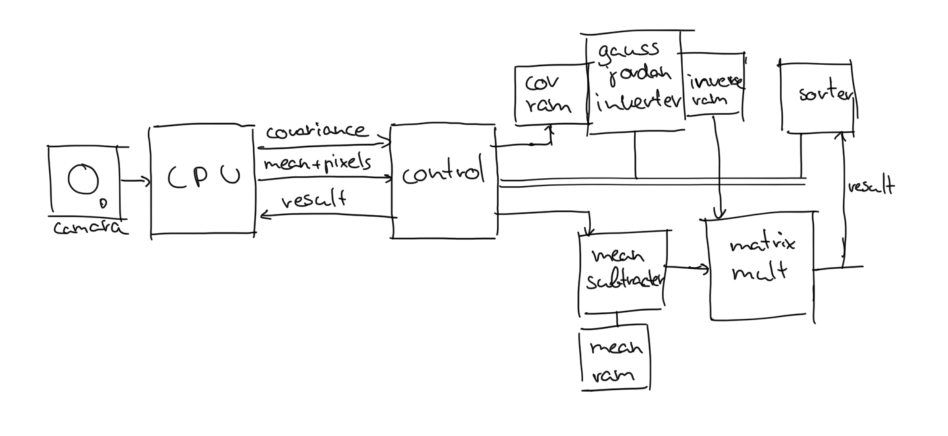
\includegraphics[height=3.5in]{figures/bus.png}


\section{Description by module}
\subsection{Control}
Este modulo actúa sobre los módulos inferiores, tanto para controlar el traspaso de datos entre ellos como para arbitrar el acceso a las RAMS y las FIFOs que comunican con la CPU.

Cabe mencionar que también realiza ciertas comprobaciones en la escritura de la covarianza para asegurar que la primera división de la inversa no se realiza con un 0, es decir, que la posición (0, 0) en la matriz de covarianzas es /= 0.
\\
\\
AQUÍ TENGO LA ELECCIÓN DE PONER UN DIAGRAMA DE ESTADOS, PSEUDOCÓDIGO O DEJARLO VACÍO
\\
\\

\subsection{Inverter}
La inversa es con diferencia el módulo más complejo y con más gasto de recursos. Además, el estudio realizado en software ha mostrado que es con diferencia el paso más susceptible a empeorar la precisión de los resultados finales. Por estas razones se ha hecho especial hincapié en su diseño.
\\
\subsubsection{Choosing the algorithm}
Antes de empezar la implementación se han estudiado varios algoritmos para realizar la inversa.
\paragraph{QR decomposition:}
La decomposición QR descompone la matriz $A$ en el producto de dos matrices $A = QR$, siendo $Q$ una matriz ortogonal y $R$ una matriz triangular superior. Con esta matriz triangular resulta sencillo calcular la inversa. Sin embargo, aunque la decomposición QR puede ser beneficiosa mientras que se cuente con un modulo de multiplicación matricial potente o varios módulos que puedan ser ejecutados de forma simultanea, como puede ser en una GPU, no aprovecha las ventajas proporcionadas por nuestro sistema como pueden ser un tamaño de matrices determinado.
\paragraph{Gauss Jordan elimination method:}
El método de Gauss Jordan dicta que si tenemos una matriz $A$ que puede ser transformada en la matriz identidad a través de operaciones elementales, estas mismas operaciones tranforman la matriz identidad en $A^{-1}$. Puesto que es posible ejecutar estas operaciones elementales en una fila entera y las operaciones entre filas son independientes, este método es fácilmente paralelizable.
Por tanto, este fue el método elegido.
\\
\\
A rasgos generales, la ejecución del algoritmo transcurre tal que:
\begin{enumerate}
\item Se genera una matriz identidad
\item Se realizan las mismas operaciones sobre ambas matrices hasta transformar la matriz $A$ en la matriz identidad
\item El resultado se encuentra en la matriz generada en el primer paso
\end{enumerate}

Estas operaciones elementales se realizan en 3 pasos, primero se transforma la matriz A en forma con triangulo superior, luego se resuelve el triangulo inferior para transformarla en diagonal y finalmente se divide la matriz entre si misma hasta conseguir la forma escalonada reducida por filas. (row canonical form)
\\
\\
\algnewcommand{\LineComment}[1]{\State \(\triangleright\) #1}
\begin{algorithm}
  \caption{Pseudocode of the Gauss Jordan method}
  \begin{algorithmic}[1]
    \Require{$A$ is a square matrix with the size $n*n$}
    \Statex
    \Function{inverse}{$A$}
      \For{$i \gets 0 \textrm{ to } n-1$} \Comment{Forward elimination to build the upper trangular matrix}
      \LineComment{row $i$ acts as the pivot}
      \If{$A[i][i] = 0$}   \Comment{If the later divisor is 0}
      	\For{$j \gets i+1 \textrm{ to } n-1$}
      		\If{$A[i][j] \neq 0$}
       			\State{$A[i] \gets A[j], A[j] \gets A[i]$}
      		\EndIf
      	\EndFor
      \EndIf
      \For{$j \gets 0 \textrm{ to } n-1$}
        \State{$A^{-1}[j] \gets A^{-1}[j]-^{-1}A[i]*A[j][i]/A[i][i]$}
        \State{$A[j] \gets A[j]-A[i]*A[j][i]/A[i][i]$}
        \Comment{These two operations may run in parallel}
      \EndFor
      \LineComment{After a complete iteration of the outer loop, the pivot contains the desired form}
      \EndFor
      \\
      \\
      \For{$i \gets n-1 \textrm{ to } 0$} \Comment{Backward elimination to build a diagonal matrix}
      \For{$j \gets i-1 \textrm{ to } 0$}
        \State{$A^{-1}[j] \gets A^{-1}[j]-^{-1}A[i]*A[j][i]/A[i][i]$}
        \State{$A[j] \gets A[j]-A[i]*A[j][i]/A[i][i]$}
        \Comment{These two operations may run in parallel}
      \EndFor
      \EndFor
      \\
      \\
      \For{$i \gets 0 \textrm{ to } n-1$} \Comment{Last division to build identity matrix}
        \State{$A^{-1}[i] \gets A^{-1}[i][i]/A[i][i]$}
        \LineComment{There is no need to update the values in the starting matrix}
      \EndFor
      \Return{$A^{-1}$}
    \EndFunction
  \end{algorithmic}
\end{algorithm}

También es posible calcular la inversa directamente para cada fila, realizando los 3 pasos seguidos, pero esta forma limita la paralelización entre diferentes filas.
\\
\\
\\

\subsubsection{Optimizaciones del algoritmo de cara a hardware}
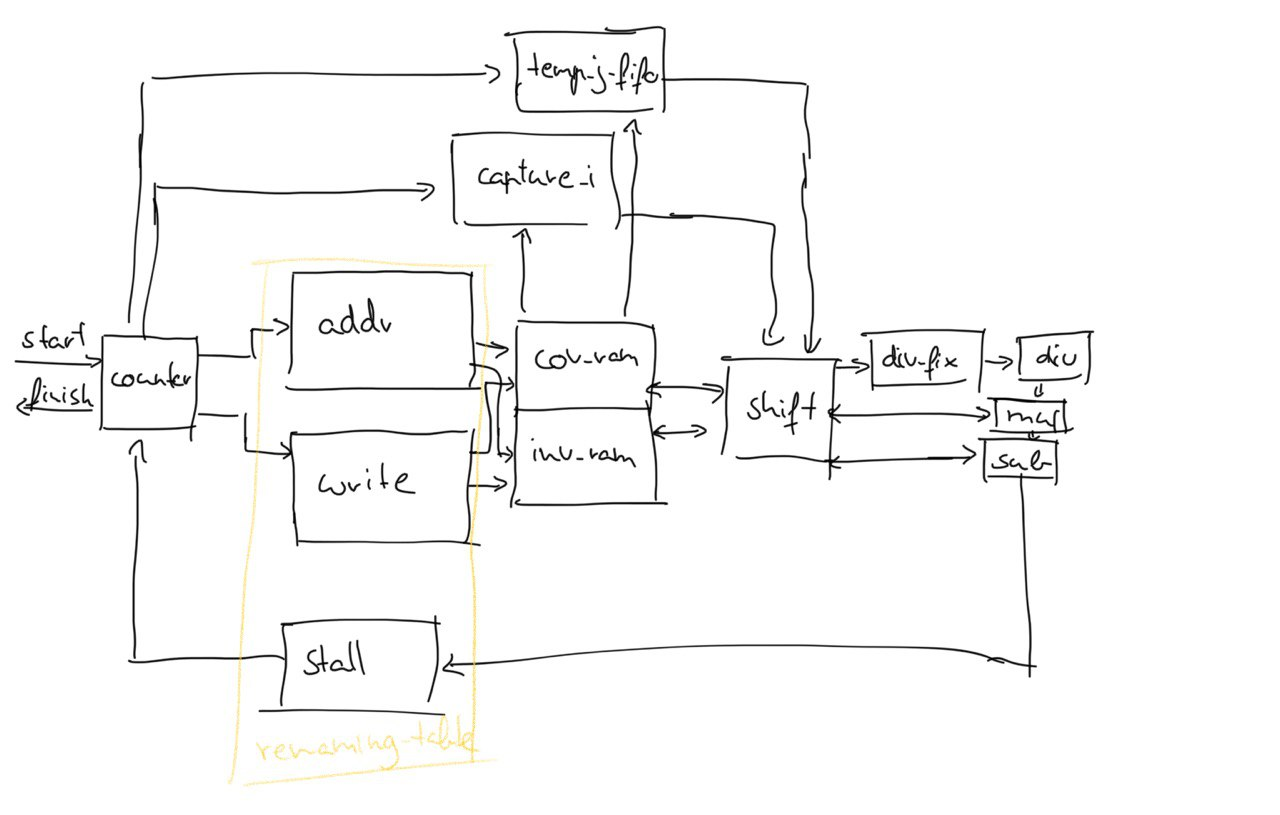
\includegraphics[height=3.5in]{figures/gauss.jpg}
\\
\\
Las operaciones a realizar en los tres pasos - triangulo, superior y diagonal- son similares, así que con el fin de ahorrar recursos se han implementado sobre la misma lógica. Existe un proceso con los contadores para controlar el orden de su ejecución.
\\
Para mejorar el rendimiento del módulo, las operaciones sobre la matriz $A$ y la matriz $A[{-1}$ se ejecutan de forma simultanea. Además, se aprovecha la segmentación de los DSP para encolar todas las operaciones consecutivas posibles. La única espera ocurre cuando se necesita el resultado de una fila para el procesado de las siguientes. Para ello, se usan varios procesos para controlar la lectura, la escritura y la captura de la fila que actuará como pivote.
\\
\\
Debería poner una rueda con colores con los cálculos que están el pipeline, los encolados, etc
\\
\\
\newcommand{\highlight}[1]{%
  \colorbox{yellow!20}{$\displaystyle#1$}}
Como se puede observar en el algoritmo, la fila [j] es usada dos momentos diferentes.
\[A^{-1}[j] \gets \highlight{A^{-1}[j]}-^{-1}A[i]*\highlight{A[j][i]}/A[i][i]\]
\\
Para poder realizar operaciones sobre filas posteriores sin retrasar lecturas, es necesario guardar este dato en una memoria auxiliar y leerlo en el momento en el que se vuelva a necesitar. Esta memoria está construida a partir de una FIFO y es controlada directamente desde el proceso contador.
\\
\\
Además, se puede observar que en el primer paso en el que se construye la matriz triangular superior, el algoritmo exige una comprobación en la fila pivote y un posible trueque de filas. Esto es necesario ya que este valor es posteriormente el dividendo, por lo que un 0 provocaría un fallo en el cálculo.
\\
Las lecturas de memoria RAM tienen un ciclo de latencia, por lo que leer un valor no adecuado dos ciclos seguidos -existiría la posibilidad de realizar un trueque de filas inplace con el pivote y la fila justo posterior- no solo añadiría latencia al cálculo si no que incrementaría la complejidad del módulo. Por lo tanto las comprobaciones del dividendo se realizan en las escrituras, y los trueques necesarios se graban en una tabla de renombrado que será leída en los cálculos posteriores. Esto permite asegurar que las lecturas van a ser siempre válidas para el cálculo. En el caso de la primera división, este dividendo viene directamente de la CPU y el módulo superior "control" se encarga de reordenar esta fila si fuera necesario.
\\
Esta tabla de renombrado se encuentra en Flip-Flops por lo que es posible acceder a ella sin ninguna latencia y al solo contener indices no sobrecarga los recursos de la FPGA. Además, esta tabla es local, por lo que los resultados tienen que ser reordenados en la propia RAM antes de salir del modulo de la inversa. Puesto que estos trueques solo ocurren en el calculo del triangulo superior, se puede aprovechar el triangulo inferior para reordenarlos. El sistema de reordenamiento es muy simple, los datos entran en el pipeline según el orden que existe en la tabla de renombrado y son escritos en su orden natural. Esto implica que los resultados de este reordenamiento van a ser correctos siempre y cuando ambas filas que hayan rotado se encuentren en el pipeline de procesado, que en el caso de  punto fijo tiene aproximadamente un tamaño de 80. Resultados experimentales muestran que rara vez hay que rotar filas -aunque lo suficiente como para ser recomendable la inclusión de un método que lidie con ello-, y que rara vez estas rotaciones exceden más una o dos posiciones en adelante.
\\
\\
En la transformación a aritmética entera se descubrió que el cálculo de la inversa es que más error llega a introducir en los resultados finales del algoritmo, por lo tanto se ha hecho estudio exhaustivo en  sobre como minimizarlo. Con la tabla de uso de los DSP [referirse a la tabla mencionada anteriormente], se ha intentado encontrar el mejor balance entre DSP y menor error introducido en la operación.
\\
Para poder aprovechar este balance, ha sido necesario reducir los valores en los que la precision limitada producía desbordamientos y aumentar valores pequeños para otorgarles más peso en las operaciones. Además, al realizar las operaciones de generación de identidad, triangulo superior, inferior y diagonal de forma independiente, se ha podido colocar diferentes desplazamientos y afinar todavía más la resolucion del algoritmo. Estas operaciones se encuentran en el proceso (shiftproc)
\\
\\
Tabla con los resultados con todo en 1, con la generacion de identidad en 29, y con todo metido. 
\\
\\
También cabe decir que existe un error en la generación de divisores de Xilinx. Cuando se introducen números cerca del limite de precision se pierde el control del signo. Por lo tanto se ha colocado un modulo antes de la división que convierte todos los operandos introducidos en positivos y guarda su posición en el pipeline. En el momento de producirse los resultados, se comprueba el tag en el pipeline, se calcula el negativo y se sustituye si es necesario.

\subsection{subtract}
El modulo de mean subtract recibe la media calculada y los pixeles originales de la imagen y los resta. Este cálculo es la deviación y aunque ya había sido calculada por la CPU, es posible que esta última deseche los datos para liberar espacio. El calculo de la media si que se requiere puesto que se supone que al ser su tamaño mucho menor, la CPU pueda mantenerlo en memoria.
El modulo recibe los elementos desde el modulo superior que los lee de una misma FIFO. Los primeros elementos son la media y son guardados en una ram que es tratada como un buffer circular, y los elementos que le siguen son restados directamente y devueltos al modulo superior de nuevo.


\subsection{Matrix multiplication}

N bandas\\
M pixeles\\
https://www.harrisgeospatial.com/docs/RXAnomalyDetection.html\\

\noindent This module performs the multiplication between the deviation and inverse matrixes.
\[ rx(x) = (x-\mu)^{T} K^{-1}_{N \times N} (x-\mu) \]


\indent \(K^{-1}_{N \times N}\) \ \ \ being the inverse matrix with a dimension of \(N \times N\),\\
\indent \((x-\mu)\) \ \	being the deviation of a pixel a dimension of \(N \times 1\) and \\			
\indent \((x-\mu)^{T}\) \ its transpose, with a dimension of \(1 \times N\).\\

The inverse gets read directly from the inverse module's output BRAM and the deviation matrix from two  FIFOS written by the CPU. The result gets written back to another FIFO.

In this step, the inverse matrix gets effectively multiplied by a unique pixel across all bands. Through row reduction, a single value for this pixel is recovered which can then be mapped to a 2d image.\\

Since the operands are heterogeneous, use is made of the associative law on matrix products that dictates that:
	\[A * (B * C) = (A * B) * C\]
	to optimize the operation.\\


\newcommand\rb{\colorbox{red!20}}
\newcommand\bb{\colorbox{blue!20}}
\newcommand\gb{\colorbox{green!20}}
\newcommand\rr{\rowcolor{red!20}}
\newcommand\br{\rowcolor{blue!20}}
\newcommand\gr{\rowcolor{green!20}}

\noindent Following will be a comparison of the first required multiplication in both methods:
\begin{quote}
	\((x-\mu)^{T} K^{-1}_{N \times N}\):	
	A row from the inverse and the whole column of the deviation get read, each element multiplied with its correspondent and all products added together. If stalls were to be avoided, this sum would need to be computed every cycle, which can easily be achieved with an adder tree.
\end{quote}

\begin{figure}[h]%t=top, b=bottom, h=here
\[
\begin{pmatrix}
\rr a & b & c \\ 
\br d & e & f \\ 
\gr g & h & i
\end{pmatrix}
*
\begin{pmatrix}
1\\
2\\
3
\end{pmatrix}
=
\begin{pmatrix}
\rr 1*a+2*b+3*c\\
\br 1*d+2*e+3*f\\
\gr 1*g+2*h+3*i
\end{pmatrix} 
\]
\caption[Optional: Short caption to appear in List of Figures]{First proposed method for the computation of a single pixel: red, blue and green represent data processed in the first, second and third cycles respectively. Note that the entire deviation data of that pixel gets used every cycle}
\end{figure}
\pagebreak
		
\begin{quote}
	\(K^{-1}_{N \times N} (x-\mu)\):
	The inverse gets also read row by row, but the deviation matrix only by elements. Each element of the first row of the matrix gets multiplied with the first element of the deviation, the result accumulated, and continued with the next pair row/element. This goes for \(N\) cycles, that is, a whole inverse matrix and a whole pixel in the deviation matrix. The result is \(N\) accumulated values which get flushed every \(N\) cycles, which ends up being the same throughput as the former method.
\end{quote}

\begin{figure}[h]%t=top, b=bottom, h=here
\[
\begin{pmatrix}
\rb1 & \bb 2 & \gb 3
\end{pmatrix}
*
\begin{pmatrix}
\rr a & b & c \\ 
\br d & e & f \\ 
\gr g & h & i
\end{pmatrix}
=
\begin{pmatrix}
\rb{1*a}+\bb{2*d}+\gb{3*g} & \rb{1*b}+\bb{2*e}+\gb{3*h} & \rb{1*c}+\bb{2*f}+\gb{3*i}
\end{pmatrix} 
\]
\caption[Optional: Short caption to appear in List of Figures]{Second proposed method: red, blue and green represent data processed in the first, second and third cycles respectively. Here only an element of the deviation data gets accessed each cycle.}
\end{figure}

While both methods have equivalent cost in time -the former has the added latency of the adder tree, the latter the latency of the accumulators- and also similar cost in DSP usage, data input by row is less taxing on the CPU and its FIFO structure can be reused for the second multiplication. Henceforth, the second approach was chosen.
\\

The second multiplication is similar in both steps, a \(1 \times N\) by \(N \times 1\) multiplication. One operand comes every cycle and each \(N\) cycles all products get added together. This sum is realized through an accumulator.\\

The module contains three subprocesses:
\begin{itemize}
	\item \emph{first\_mac} reads the inverse and performs its multiplication with the first FIFO. The products are then accumulated till a whole pixel has been computed.
	\item \emph{second\_mac} stores the results of \emph{first\_mac} in registers and performs the multiplication with the second FIFO, with the result being accumulated. Every cycle, the registers are shifted so a new multiplication is done.
	\item \emph{write\_proc} controls the writing of the results from \emph{second\_mac} to the result FIFO.
\end{itemize}



\subsection{sorter}
 El sorter recibe un valor y un par de coordenadas cada nbandas ciclos. Estos valores son escritos en una memoria ram que actua como una lista ordenada. Cada valor introducido es comparado con la cabeza de la lista, el valor más alto guardado y el otro es guardado en una variable temporal y comparada con el segundo valor en la lista, así sucesivamente. Puesto que se recibe un valor cada nbandas, el numero maximo de valores posibles a almacenar en esta lista es también nbandas. El resto de valores son deshechados. Cuando se ha introducido el ultimo valor, el modulo comunica los pixeles más altos, es decir, más anomalos, al modulo superior para que estos sean comunicados a la cpu.
\section{ejecucion paso a paso}
que tengo que poner aqui

